We created the topology shown in Figure~\ref{fig:topology} in ExoGENI to conduct our experiments. Among the $23$ nodes in this topology, we specify $6$ data origins and $6$ data sinks as the end hosts 
to transfer a batch of data files ($886$ files) of different sizes that we randomly acquired from OSG. There are $49$ links in total with which we try to emulate a topology following the power law, i.e., $4$ routing 
nodes in the middle to emulate the backbone domains and the rest emulate the access domains in between the backbone nodes and the end hosts. 

We ran two sets of experiments to collect two sets of raw training data. In the first one, called {\it Partial},
data transfers only happen between the origins and sinks, where every origin node sends all the $886$ files 
to all the receiving nodes in parallel. In the second one, called {\it Complete}, data transfers happen between all the end host pairs. 
We further parallelized the data transfer process to reduce the emulation time down to about twenty four hours for this particular network.  

The file integrity is being checked at the receiving end host and each file transfer accounts for one data flow and therefore a
 data sample in a training data set.

For each experiment, probabilistic integrity error or network impairment via the Chaos Jungle tool is injected to the $54$ link interfaces and $12$ end hosts in sequence with the given probability setting. 
For each fault injection scenario, the entire set of {\it Partial} or {\it Complete} data transfers are conducted. Each link interface or node component with fault injected represents a label.  
The receiving node checks if a received file is identical to its original copy via checksum and marks this data transfer as a failure data sample if checksums do not match. 
We treat retransmission as a separate feature for the data samples.  A file could also be missed at the destination due to ultimate transfer failure which is also treated as a failure. 
If the checksum matches, this data transfer becomes a success data sample in the training data set. Otherwise, it is labeled by the corresponding faulty element, one of the total $66$ labels in this study. 
As a very basic benchmark, we note the accuracy of random classification would be merely $\frac{1}{66}$.

Through extensive data analysis, we achieved three import goals in our RCA study:  (1) performance comparison in terms of accuracy and training time performance of different models, 
(2) impact quantification of different types of features on the model performance, esp. the file size the transfer throughput, (3) handling of the inherited data imbalance in the training data set.

Following figures show the overall performance results when using the three chosen models as presented in Section~\ref{sec:ml}. We use One Hot Encoding for all the categorical features. 
The figures from Random Forest and Bayes models have two parts: the left part shows the results for the {\it Partial} data set and the right part shows the results for the {\it Complete} data set. 
The results from the SVM show two different types of models: linear SVM and general SVM with RBF kernel. Each part depicts three types of prediction performance metrics: Per Flow Accuracy, 
Per Flow F!-Score, and $Top-k$ Aggregate Flow Accuracy with $k=1,2,3$.

\begin{figure}[!ht]
\begin{center}
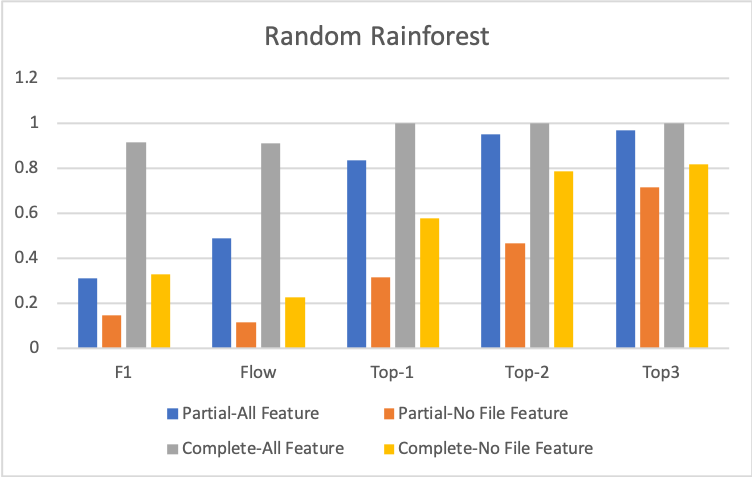
\includegraphics[width=0.45\textwidth]{./figure/rf-accuracy}
\end{center}
\vspace{-0.05in}
\caption{Classification Accuracy with Random Forest Model}
\vspace{-0.05in}
\label{fig:dt}
\end{figure}

Fig.~\ref{fig:dt} presents the results using the random forest model. The single flow level accuracy is very poor and the accuracy increases dramatically with bigger $k$. It also clearly shows that the model with {\it Complete} data performs much better than the {\it Partial} case. However, the gap becomes small when $k=3$. 

\begin{figure}[!ht]
\begin{center}
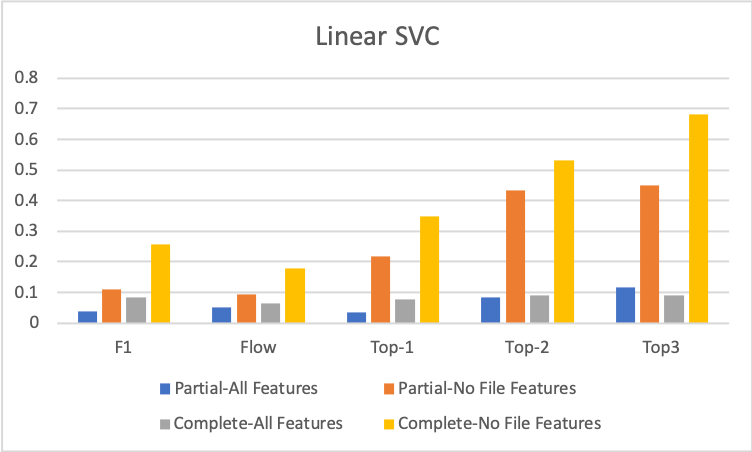
\includegraphics[width=0.45\textwidth]{./figure/svc-accuracy}
\end{center}
\vspace{-0.05in}
\caption{Classification Accuracy with SVM Model}
\vspace{-0.05in}
\label{fig:svm}
\end{figure}

Fig.~\ref{fig:svm} depicts the results using two different models: linear and general SVM with RBF kernel. It shows the same trends with regards to $k$. It also clearly shows that Linear SVM performs better than the general SVM.
\begin{figure}[!ht]
\begin{center}
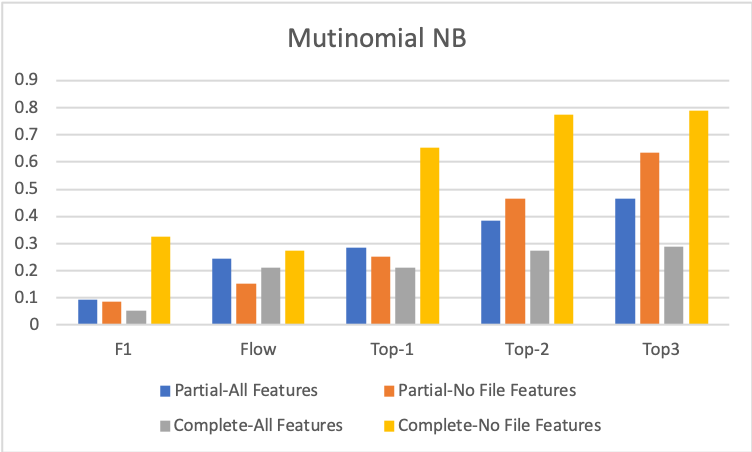
\includegraphics[width=0.45\textwidth]{./figure/nb-accuracy}
\end{center}
\vspace{-0.05in}
\caption{Classification Accuracy with Multinomial Naive Bayes}
\vspace{-0.05in}
\label{fig:bn}
\end{figure}

Fig.~\ref{fig:bn} shows the results using the Multinomial Naive Bayes approach. Again, the accuracy increases with $k$.

When comparing between above three models, the random forest performs the best, linear SVM the next best, and the Bayes model performs the worst. 

When $k=3$, the maximal achieved accuracy is slightly above $80\%$, which is very promising for our specific network RCA problem. We tried larger values of $k$. The accuracy doesn't change much until $k$ reaches 20, when it will jump to above $90\%$. We believe the accuracy stall may be mainly due to the particular topology and more importantly the set of the end hosts for data transfers that do not include all the router nodes, which violates the necessary condition to cover all the possible failure causes in a network~\cite{netbouncer:nsdi18}.  

%\begin{comment}
We next look into the training time of the above three models. From Table.~\ref{tab:time}, it is clear that SVM takes significantly longer time than the other two. Actually the SVC with the default RBF kernel takes much longer time than the linear SVC whose running time is shown in the table. Between the other two, the decision tree model takes the shortest time. Another observation is that the training with the {\it Complete} data set finishes much faster than that with {\it Partial} data set. This makes sense because more complete training data helps the model training converge faster. 

To make the evaluation complete, we also present the F-Score for the single label classification {\it Complete} case in the same table. The SVM model gets the best F-score. As we stated before, we believe the accuracy is the more meaningful metric for the RCA problem, though we will continue to explore better metrics.     
\begin{table}[!ht]
\caption{Training Time and F\-Score}
\label{tab:time}
%\vspace{-0.1in}
\begin{center}
\begin{tabular}{ |c|c|c|c| } 
 \hline
  & Partial & Complete & F-Score ($k=1$)\\ 
 \hline\hline
 Decision Tree & 164ms & 95.1ms & 0.3266\\ 
 \hline
 Bayes & 416ms & 174ms & 0.3382 \\
 \hline
 SVM & 26700ms & 10300ms & 0.368 \\ 
 \hline
\end{tabular}
\end{center}
%\vspace{-0.1in}
\end{table}
Combining both training accuracy and training time, the random forest model appears to be a clear winner for the studied RCA problem. Therefore, in the following analysis, we focus on this model.
%\end{comment}

In order to gain more insight into the classification accuracy performance, we observed that the majority mislabeled data in the prediction are those with labels of end host faults.  This is because the raw training data set is highly imbalanced due to the different impacts of the injected failures on the data files being transferred~\ref{sub:ml:imbalance}. There are significantly less integrity errors caused by the faulty end hosts, \ie, significantly less labeled data in these classes.

The details are shown in Table~\ref{tab:class}. We first categorize all the labeled data into two groups: those with faulty link interfaces and those with faulty end hosts, {\it Max} and {\it Min} represent the maximum and minimum number of samples in a class in each category, and the $Top-k$ up to $k=3$ accuracy under each category is calculated separately. We can see that there are hundred times more samples in a few link failure classes than those in all the end host failure classes, and samples from some link failures classes are about ten times less than those from some other link failure classes. As a result, all the end host failures are misclassified in all the cases, while most link failure cases are correctly classified and the accuracy reaches $1$ when $k=3$.

\begin{table}[!ht]
\caption{Classification Accuracy Differentiation}
\label{tab:class}
%\vspace{-0.1in}
\begin{center}
\begin{tabular}{ |c|c|c|c|c| } 
 \hline
  \multicolumn{5}{|c|}{Link Faults} \\
 \hline
 Max & Min & $Top-1$ & $Top-2$ & $Top-3$\\ 
 \hline
 1443 & 121  & 0.0.74 &  0.79 & 0.98 \\
 \hline
\end{tabular}

\begin{tabular}{ |c|c|c|c|c|} 
 \hline
\multicolumn{5}{|c|}{Host Faults} \\
 \hline
 Max & Min & $Top-1$ & $Top-2$ & $Top-3$ \\ 
 \hline
11 & 11  & 0 &  0 & 0\\
  \hline
\end{tabular}
\end{center}
%\vspace{-0.1in}
\end{table}

The main techniques to solve the dataset imbalance problem are to rebalance the data via oversampling or downsampling data from different classes. Since the labeled data subsets from the end host failure classes are rather small, the downsampling techniques will not improve on the model performance. We therefore focus on studying three representative oversampling techniques: random, SMOTE, and ADASYN.

The random oversampling approach is straightforward in which new samples are randomly generated by copying the existing samples from the undersampled classes. In our case, the resulted augmented data set will have 1443 labeled data for each of the 66 classes. 

The SMOTE(Synthetic Minority Oversampling Technique ) ~\cite{smote:2002} and the ADASYN (Adaptive synthetic sampling approach for imbalanced learning)~cite{ADASYN:2008} methods are two popular oversampling techniques that 
generate new samples by interpolation rather than duplication of existing samples using variants of k-Nearest Neighbors classifier method.


